% % $RCSfile: proj_proposal.tex,v $
% % $Revision: 1.3 $
% % $Date: 2016/06/10 03:44:08 $
% % $Author: kevin $

\documentclass[11pt, a4paper, twoside, openright]{report}

\usepackage{float} % lets you have non-floating floats
\usepackage{url} % for typesetting urls
\usepackage{graphicx}
\usepackage{subcaption}
\usepackage{hyperref}

\renewcommand{\thesection}{\arabic{section}}

%  We don't want figures to float so we define
%
\newfloat{fig}{thp}{lof}[chapter]
\floatname{fig}{Figure}

% % These are standard LaTeX definitions for the document
% %
\title{Instrumentation System for Liquid Drop Impact and Evaporation}
\author{Daniel Eisen}

% % This file can be used for creating a wide range of reports
% %  across various Schools
% %
% % Set up some things, mostly for the front page, for your specific document
%
% Current options are:
% [ecs|msor|sms]          Which school you are in.
%                         (msor option retained for reproducing old data)
% [bschonscomp|mcompsci]  Which degree you are doing
%                          You can also specify any other degree by name
%                          (see below)
% [font|image]            Use a font or an image for the VUW logo
%                          The font option will only work on ECS systems
%
\usepackage[image,ecs]{vuwproject} 

% You should specifiy your supervisor here with
\supervisor{Gideon Gouws}
% use \supervisors if there are more than one supervisor
\otherdegree{Bachelor of Engineering with Honours}
% Unless you've used the bschonscomp or mcompsci
%  options above use
%   \otherdegree{OTHER DEGREE OR DIPLOMA NAME}
% here to specify degree

% Comment this out if you want the date printed.
\date{}

\begin{document}

% Make the page numbering roman, until after the contents, etc.
\frontmatter

% %% %% %% %% %% %% %% %% %% %% %% %% %% %% %% %% %% %% %% %% %% %% %% %% %% %% %%

\begin{abstract}
\end{abstract}

% %% %% %% %% %% %% %% %% %% %% %% %% %% %% %% %% %% %% %% %% %% %% %% %% %% %% %%

\maketitle
\tableofcontents

% we want a list of the figures we defined
%\listof{fig}{Figures}

% %% %% %% %% %% %% %% %% %% %% %% %% %% %% %% %% %% %% %% %% %% %% %% %% %% %% %%

\mainmatter

% %% %% %% %% %% %% %% %% %% %% %% %% %% %% %% %% %% %% %% %% %% %% %% %% %% %% %%

\section{Introduction}
\textit{Will be an executive summery of following sections, mention who's research this fits into, requirement for budget to cover manufacturing cost etc, and that Will will be a contributor to an auxiliary project that affects this.}






\section{The Problem}
This project is concerned with the development of a instrumentation rig for the study of droplet impact and drying. It is primarily/initially motivated by the powdered milk production process, specifically the behaviour of the drying and collision of concentrated milk droplets. Furthermore, the research, and developed method and procedure can be applicable to various industries. \\

To effectively investigate the behaviour, a variety of aspects can be tracked and characterised during a microscale equivalent lab process, from differing temperatures, substrates, volume, and concentrations. \\

Currently there is an existing platform for the dispensing of droplets and data capture using high speed cameras and other various sensors. It has limitations due to manual control of starting the cameras capture and temperature capturing as well as requiring the operator to position and dispense the droplet by hand. \\

This project will therefore, focus on the development of the third generation of this platform with the aim to design and integrate various new subsystems and evaluate their performance against the existing platform with the main project goal of having a more stable, repeatable testing platform that will not only yield more usable data but streamline the experimental process.

\subsection{Existing Process}
The current procedure as of the project beginning is a manual process. There is currently no securing bracket of any kind for the substrate sample and heater stack, the cameras and other sensors are turned on one by one and most importantly the droplet is rotated above a mark in the substrate and dispensed via syringe by hand.

The droplet then falls onto the substrate, monitored by 2 high speed cameras (profile and overhead) and the temperature of the substrate is measured via an embedded thermocouple camera a time series waveform of the experiment.

We hypothesis that this method contributes a large amount of variation into the collected data that could be masking the parameter space of interest, and limiting the granularity at which conclusions can be drawn about process of impact and evaporation.

\newpage
\section{Proposed Solution}
The primary driving principle for both the design and evaluation of this next generation is a focus on \textit{increasing reliability of the process by designing new and/or improving existing subsystems of the rig}. 

To be able to quantify success in that aspect and evaluations of current systems results is needed to  identify its short comings. Therefore, one of the first steps is to produce an report detailing such aspects.
\begin{itemize}
  \item Repeatability of dispensed droplet parameters (position, volume (size), contact angle) and correlate and/or see how the variation in these parameters effects the observed temperature profile and physical behaviours of the droplet throughout the evaporation process.
  \item Identify other sources of variation, such as humidity etc and their weight of influence (whether perusing a solution is worthwhile)
  \item Compare with similar solutions in literature to gain more insight into required design consideration and constraints.
\end{itemize}

Alongside this, the first step is a mechanical design of a bracket and clamp assembly to hold and centre a aluminium heatspeader, Peltier heater, and substrate to the sample stage (fig \ref{fig::old_rig}).

From this, the primary effort will go into the droplet dispensing stage. Possibly integrating an electronic pipette and motorised stage XY  rotation to address the consistency problems. Constraints that will have to be overcame are the reduce volume capacity (syringe: ~12-15ml to max 10ml) and refilling from a reservoir.

The above represent the base deliverables, but the project may be extended with data collection automation and synchronisation, and more environmental monitoring and control.

\begin{figure}
  \begin{subfigure}{.5\textwidth}
    \centering
    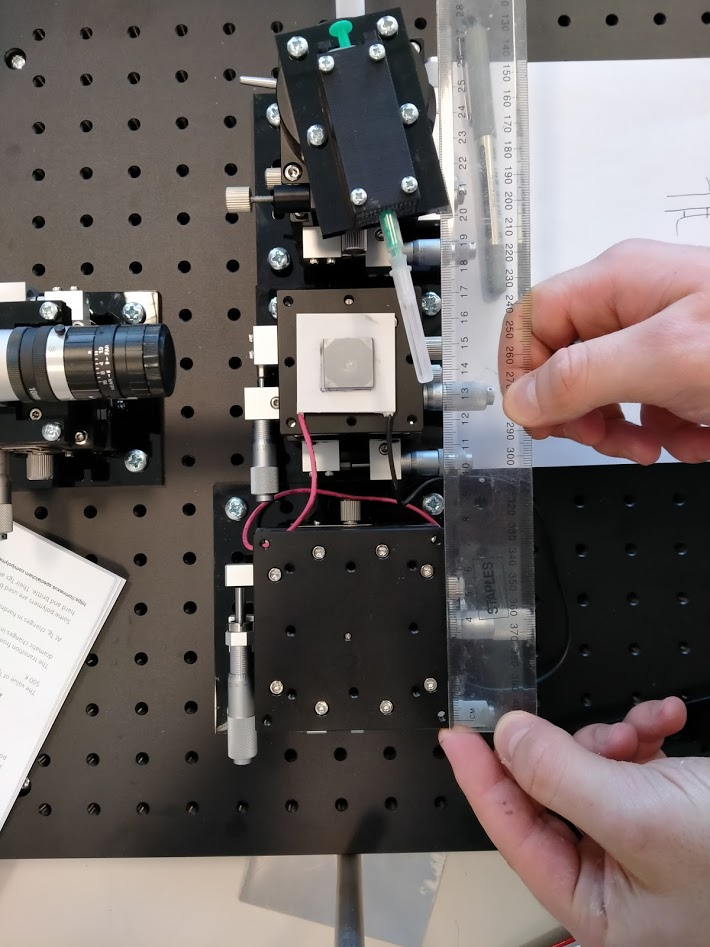
\includegraphics[height=.5\linewidth]{Figures/Full_rig_top.jpg}
    \caption{Full Top View}
  \end{subfigure}%
  \begin{subfigure}{.5\textwidth}
    \centering
    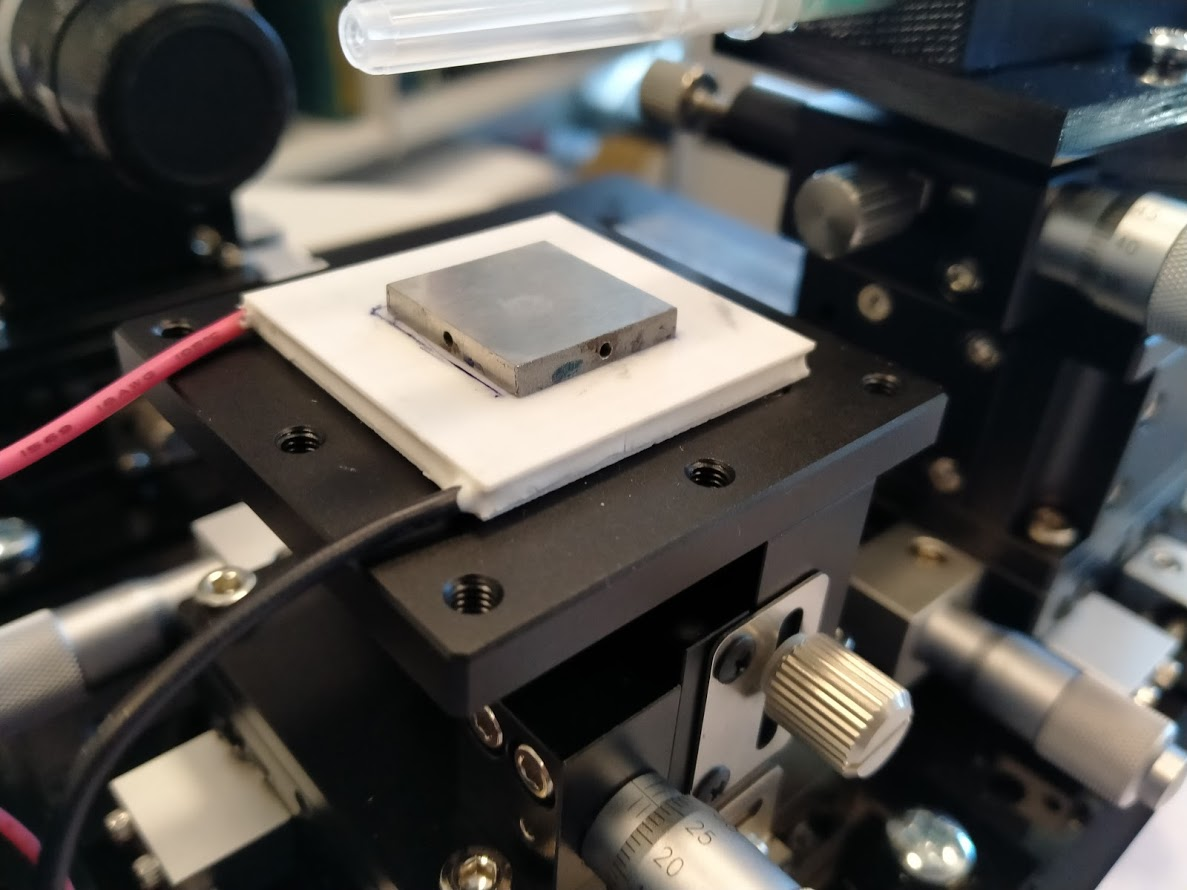
\includegraphics[height=.5\linewidth]{Figures/substrate_stack.jpg}
    \caption{Substrate Stack close-up}
  \end{subfigure}
  \caption{Previous Rig Assembly (bar top camera)}
  \label{fig::old_rig}
\end{figure}


\subsection{Base Deliverables}
\begin{itemize}
  \item Mechanical designs to hold, centre, and clamp the substrate stack  together (1-2 weeks).
  \item Produce evaluation document based on generation 2 performance (2-3 weeks)
  \item (Main) Improved Droplet Delivery stage; dispensing control, motorised stage.
\end{itemize}

\subsection{Stretch Goals}
\begin{itemize}
  \item Synchronous data collection, i.e. cameras, temperature, droplet
  \item Measure and control environmental factors
\end{itemize}

\subsection{Timeline}
\begin{figure}[h]
  \centering
  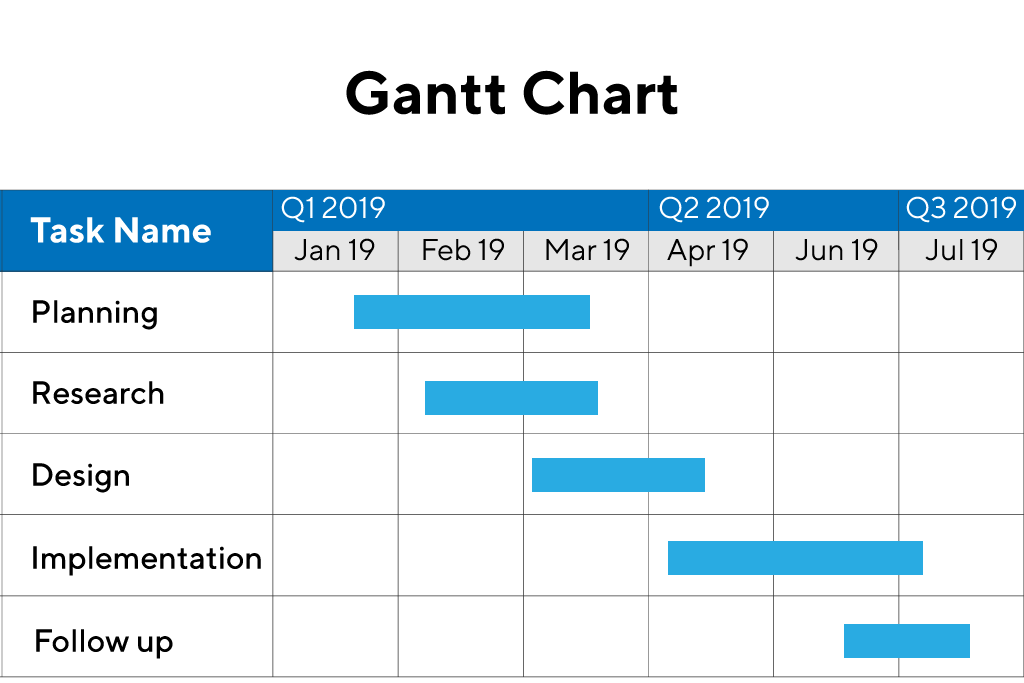
\includegraphics[width=\textwidth]{Figures/Gantt-chart_filler.png}
\end{figure}

\newpage
\section{Evaluating your Solution}
To evaluate the success, the produced evaluation document on generation 2 will serve as the primary comparison. Each subsystem; mechanical brackets, droplet dispensing, temperature measurements will be tested individually to quantise their contribution and as a gradually integrated whole.

The preliminary evaluation criteria (subject  to change with the discretion of the previous generation analysis) include consistency and repeatability of the following:
\begin{itemize}
  \item Dispensed volume
  \item Impact characteristics (centre, angle, etc)
  \item Uncontrolled temperature variation
\end{itemize}



\section{Resource Requirements}

\subsection{Facilities and Tools}
\begin{itemize}
  \item Labs AM219 and LB207
  \item Computer with SolidWorks, LabView, and other data processing tools
  \item Electronics Test bench (PSU, signal generator, scope etc)
  \item Access to fabrication workshop
\end{itemize}

\subsection{Health and Safety}
The project does not necessitate
\begin{itemize}
  \item Lab Induction (LM207)
  \item Peltier Heaters
  \item Basic electronic safety
\end{itemize}


\subsection{Budget}
It is worth noting that the instrumentation platform is largely constructed with all its major components, and most needed parts for the design and development of the project are already present.

Given this, the project has estimated a budgetary restriction of \$400.
\begin{itemize}
  \item \$200 to cover workshop manufacturing costs of mechanical designs
  \item \$200 for the purchase stepper motors and auxiliary components, PCB design and manufacture and all other electronic component costing.
\end{itemize}

\section{COVID-19 Alert Level Management}


% %% %% %% %% %% %% %% %% %% %% %% %% %% %% %% %% %% %% %% %% %% %% %% %% %% %% %%
\backmatter
% %% %% %% %% %% %% %% %% %% %% %% %% %% %% %% %% %% %% %% %% %% %% %% %% %% %% %%

\nocite{*}
\bibliographystyle{ieeetr}
\bibliography{sample}
\end{document}
